\documentclass[10pt, oneside]{article} 

\usepackage{amsmath, amsthm, amssymb,amsfonts,appendix}
\usepackage{bbm, bm,booktabs}
\usepackage{calrsfs,color,cite,caption}
\usepackage{esint,enumitem}
\usepackage{fancyhdr,fontspec,float}
\usepackage{graphicx,graphics,geometry}
\usepackage{indentfirst}
\usepackage[labelfont=bf]{caption}
\usepackage{mathptmx}
\usepackage{stmaryrd,siunitx,subfigure,setspace}
\usepackage[stable]{footmisc}
\usepackage{tikz,textcomp}
\usetikzlibrary{fit,positioning,arrows,automata}
\usepackage{verbatim}
\usepackage{wasysym}
\usepackage{wrapfig}



\geometry{tmargin=.75in, bmargin=.75in, lmargin=.75in, rmargin = .75in}  



\newtheorem{thm}{Theorem}
\newtheorem{defn}{Definition}
\newtheorem{conv}{Convention}
\newtheorem{rem}{Remark}
\newtheorem{lem}{Lemma}
\newtheorem{cor}{Corollary}


\title{
Pattern Recognition HW 1
}
\author{171240510 Yuheng Ma\\[0.3cm]{Math Major, Kuang Yaming Honors School}}
\date

\begin{document}

\maketitle

\vspace{.25in}
\section{01 Introduction}
\begin{enumerate}
	\item We need $\sqrt{\frac{8a-1}{3}}>0$ and thus $a>\frac{1}{8}$.
	\item 1
	\item a=$\frac{1}{2}$, where output value is 1. It might be constantly 1.
	\item 1.3956439237389602+0.2284251258739286j
	\item use $$\sqrt[3]{a+\frac{a+1}{3} \sqrt{\frac{8 a-1}{3}}}+sign(a-\frac{a+1}{3} \sqrt{\frac{8 a-1}{3}})\sqrt[3]{|a-\frac{a+1}{3} \sqrt{\frac{8 a-1}{3}}|}$$
	\item For any a$\in \mathbb{R}$, $\sqrt[3]{a+\frac{a+1}{3} \sqrt{\frac{8 a-1}{3}}}+\sqrt[3]{a-\frac{a+1}{3} \sqrt{\frac{8 a-1}{3}}}=1$.\\\textbf{Proof:} After some algebra, we have
	$$
	\sqrt[3]{a+\frac{a+1}{3} \sqrt{\frac{8 a-1}{3}}}+\sqrt[3]{a-\frac{a+1}{3} \sqrt{\frac{8 a-1}{3}}}=\frac{\sqrt[3]{(1+\sqrt{\frac{8a-1}{3}})^3}+\sqrt[3]{(1+\sqrt{\frac{8a-1}{3}})^3}}{2}
	$$
	and thus proved.
	\item Take a=2, we have $$\sqrt[3]{2+\sqrt{5}}+\sqrt[3]{2-\sqrt{5}}=1$$
	\item Cardano stated that $$
	\sqrt[3]{-\frac{q}{2}+\sqrt{\frac{q^{2}}{4}+\frac{p^{3}}{27}}}+\sqrt[3]{-\frac{q}{2}-\sqrt{\frac{q^{2}}{4}+\frac{p^{3}}{27}}}
	$$
	is a root of $x^3+px+q$ while $4 p^{3}+27 q^{2}>0$. Thus when 1 is a root of $x^3+px+q$, we have p+q=-1. Then$$
	\begin{aligned}
	&\sqrt[3]{-\frac{q}{2}+\sqrt{\frac{q^{2}}{4}+\frac{p^{3}}{27}}}+\sqrt[3]{-\frac{q}{2}-\sqrt{\frac{q^{2}}{4}+\frac{p^{3}}{27}}}\\
	=&\sqrt[3]{-\frac{q}{2}+\sqrt{-\frac{q^{3}}{27}+\frac{5}{36} q^{2}-\frac{q}{9}-\frac{1}{27}}}+\sqrt[3]{-\frac{q}{2}-\sqrt{-\frac{q^{3}}{27}+\frac{5}{36} q^{2}-\frac{q}{9}-\frac{1}{27}}}
	\end{aligned}
	$$
	By replacing q by -2a, we have Equation 1. Also, by $$-\frac{q^{3}}{-27}+\frac{5}{36} q^{2}-\frac{q}{9}-\frac{1}{27}=-\frac{(q/2-1)^2}{9}\frac{4q+1}{3}$$, we can see that constraint of q is q<$-\frac{1}{4}$ which is just a>$\frac{1}{8}$.
\end{enumerate}

\section{02 Math 1}
\begin{enumerate}
	\item $(\frac{\sqrt{3}}{2},\frac{3}{2})$
	\item$ \left(\boldsymbol{x}-\boldsymbol{x}_{\perp}\right) \cdot \boldsymbol{y}$=$(\frac{\sqrt{3}}{2},-\frac{1}{2})\cdot(1,\sqrt{3})$=0
	\item As below
	\begin{figure}[H]
		\centering
		
		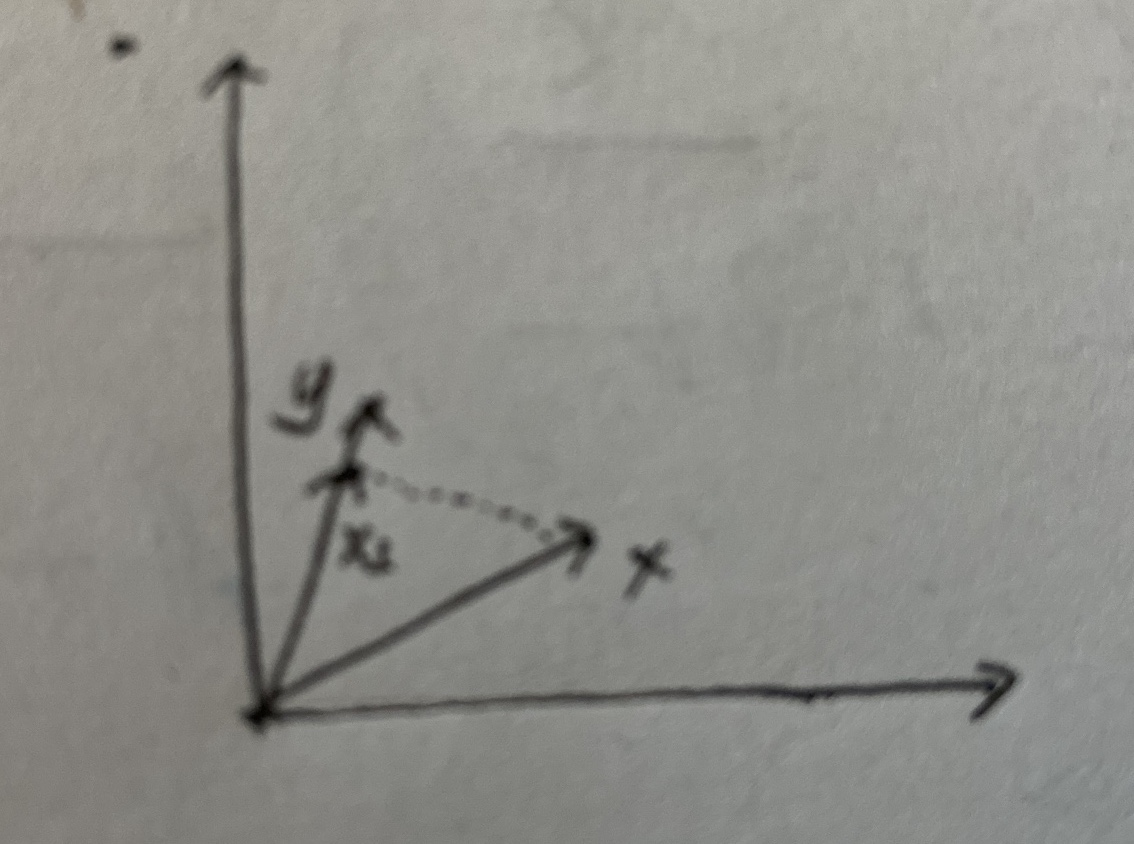
\includegraphics[width=0.5\linewidth]{1.jpeg}
		\label{1}
	\end{figure}
	\item By hint $$\left\|\boldsymbol{x}-\boldsymbol{x}_{\perp}\right\|^{2}+\left\|\boldsymbol{x}_{\perp}-\lambda \boldsymbol{y}\right\|^{2}=\|\boldsymbol{x}-\lambda \boldsymbol{y}\|^{2}$$ the inequality holds natually and equals when $x_{\perp}=\lambda y$
\end{enumerate}

\section{02 Math 2}
\begin{enumerate}
	\item x>0
	\item 6
\end{enumerate}

\section{02 Math 6}
\begin{enumerate}
	\item $E(x)=\beta^{-1}, Var(x)=\beta^{-1}.$
	\item c(x)=$1-e^{-\beta x}$
	\item $$
	\begin{aligned}
		P(X \geq a+b | X \geq a)=&\frac{P(X\geq a+b, X\geq a)}{X \geq a}\\
		=&\frac{P(X\geq a+b)}{X \geq a}\\
		=&\frac{1-c(a+b)}{1-c(a)}\\
		=&e^{-\beta b}\\
		=& P(X\geq b)
	\end{aligned}
	$$
	\item 1000, 1000.
\end{enumerate}

\section{02 Math 10}
\begin{enumerate}
	\item f is smooth and f''(x)=$a^2e^{ax}$>0, thus convex.
	\item g is smooth and g''(x)=$-\frac{1}{x^2}$<0, thus concave.
	\item h is convex on (0,+$\infty$). When $x_1$=0, $$
	\frac{x_1+x_2}{2}\log(\frac{x_1+x_2}{2})=\frac{x_2}{2}\log(\frac{x_2}{2})>\frac{x_2}{2}\log x_2=\frac{x_1\log x_1 +x_2 \log x_2}{2}
	$$
	Thus the inequality hold for $x_1, x_2\in [0,+\infty)$
	\item Since $p_i$s are probabilities, $$
	L(p)=H-\lambda(\sum p_i-1)$$
	$$
	\frac{\partial L}{\partial p_i}=-log_2p_i -\lambda-\frac{1}{\log 2}, i=1,\cdots, n
	$$
	Thus if partial derivatives all equal 0, $p_i$s are equal, which is $p_i=\frac{1}{n}$.
\end{enumerate}
\end{document}
